\section{Image Generation}
Originally, when you wanted to create e.g. a new chairstyle, you had to retrain the whole network. However, through Encoder-Decoder networks it became possible to only having to train once for different input images. These single-to-multi view architectures take in an input image of the object and an arbitrary desired output view and to create this output view plus additional depth map (U-Net like). Outputs were often blurry due to uncertainty.

\subsection{3D Shape Prediction}
The goal of this task is to create the 3D shape of an object from a single input image.\\

\b{Octree Generating Networks (OGN)\\[.5em]}
Octrees are a datastructure used to split 3D data into structured 3D grids. The initial representation (root) consists of a single cube. This cube is then recursively split into eight smaller cubes (successors) until you run out of memory.\\

The challenge is to build a decoder which is able to produce octree structures of different resolutions. In practice this is done by stacking OGN layers. Each layer gets told by the previous layer which cubes are to be further refined. The layer then refines these cubes and afterwards decides which cubes are still relevant for the next layer. You do this until you are at the desired resolution.\\

\b{Note:} Since only few cubes are of interest, the sparse feature maps are implemented using hash functions. In comparison to using dense feature maps, OGN scales a lot better with higher resolutions.\\

\b{Note:} Networks mainly run a classifier on the input image and provide the best matching linear combination of training shapes.

\subsection{Variational Autoencoders}
\b{Important:} For details see DL summary!\\

VAEs are probabilistic generative models for modelling a data distribution. The encoder maps from the complex input distribution to a simpler latent space (typically Gaussian), while the decoder maps from the latent space to the original distribution (see next image).\\
Both encoder and decoder are learned by optimizing the ELBO:
\cf{
    \fL_{\theta,\Phi}(x) = \mathbb{E}_{q_\Phi(z|x)}[\log p_\theta(x,z)-\log q_\Phi(z|x)]
}
\begin{figure}[ht!]
    \centering
    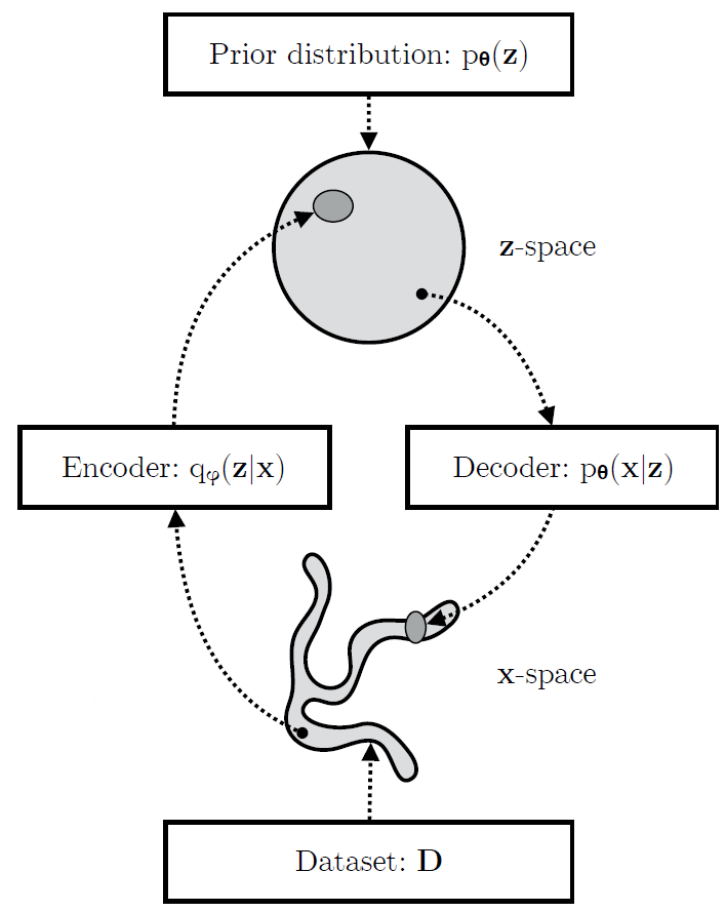
\includegraphics[scale=0.55]{vae.png}
\end{figure}

\subsection{Generative Adversarial Networks}
The goal of GANs is to model a data distribution with a generator. You can do that by forcing the generated samples to fit the data distribution by jointly training the discriminator, which tries to distinguish the generated samples from the target distribution. Generator maps from samples of a base distribution to samples of a target distribution and tries to fool the discriminator.\\
While training you alternatingly train the generator and discriminator in an unsupervised fashion.\\

Major problems are:
\begin{itemize}
    \item Tricky training (due to alternation, must keep equilibrium)
    \item Mode collaps (generator may generate only a small subset of distribution)
\end{itemize}

\newpage

\b{Style GANs\\[.5em]}
Style GANs try to control the image generation by a condition z (e.g. predefined style). The latent vector \f{z} is transformed into a vector \f{w} that is converted into a learned affine transformation (style).\\
This can for example be used to morph the styles of two different image sources.

\subsection{Diffusion Models}
The task is to learn to predict the small steps that turn a noisy image into a slightly less noisy image. The training data can be generated by iteratively adding Gaussian noise to the training images (self-supervised learning). Image generation starts from pure noise and iterates back towards a clean image.\\

\b{Conditioning the Diffusion Process\\[0.5em]}
Instead of modeling the unconditional mapping, the network (U-Net like) must take a condition \f{y} and produce the reverse noise based on that condition: \f{\nabla_x\log p(x|y)}. Via Bayes' rule, we get:
\cf{
    \nabla_x \log p(x|y) = \nabla_x \log p(y|x) + \nabla_x \log p(x)
}
which translates to:
\cf{
    \text{conditional diffusion step} = \text{predictive distr. (e.g. classifier)} + \text{unconditional diffusion step}.
}
The nice thing here is that this conditional can be added post-hoc, meaning after model training. However, classifiers are not made for noisy images, so the gradient is often bad.\\
Alternatively, we can of course directly train a conditional diffusion model. In practice, the condition is sometimes dropped during training so that the model also learns the unconditional distribution.\\ \f{\to} This leads to much better results.\\

\b{Note:} We cannot just use an unconditional model and adapt it, but require training on the target distribution of conditioned data. BUT: The unconditional model can be used as initialization.

\newpage

\subsection{Final Remarks}
\begin{itemize}
    \item Direct decoder models are notprobabilistic, but most straightforward
    \item GANs, VAEs, and diffusion modelshave probabilistic components
    \item To control what is being generated, some conditioning is needed. Typically this is handled by training with an appropriate conditional distribution.
\end{itemize}
\vspace{2cm}
\begin{figure}[h!]
    \centering
    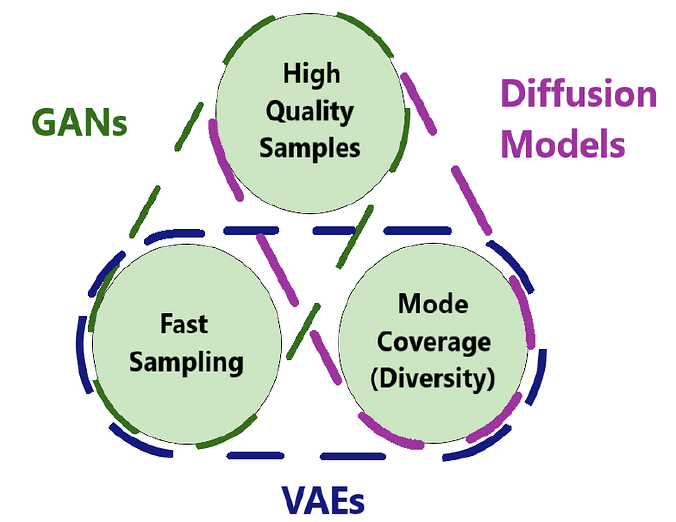
\includegraphics[width=0.5\textwidth]{gen.png}
\end{figure}







\newpage